% Ejercicio 9, inciso c) — issue #3. Mismo contenido que inciso-c.md.
% Fragmento sin preámbulo: lo incluye latex/main.tex, que ya pone el título del inciso.

\begin{quote}
\itshape
¿Qué pasa si un cliente no puede ser notificado? ¿Cómo evitar bloquear el hilo principal?
¿Observer es síncrono o asíncrono?
\end{quote}

Las tres preguntas se responden sobre el código del inciso b. Nada de lo que se afirma aquí
se queda en la teoría: cada punto tiene su demostración ejecutable y su prueba unitaria.

\begin{lstlisting}[language={}, numbers=none, basicstyle=\ttfamily\footnotesize, columns=fullflexible, keepspaces=true]
cd codigo
dotnet run --project Bolsa.Notificaciones -- asincrono   # la demostración de este inciso
dotnet test                                              # 20 pruebas, 9 de este inciso
\end{lstlisting}

\begin{table}[H]
\centering
\small
\begin{tabularx}{\textwidth}{>{\raggedright\arraybackslash}p{4.3cm} >{\raggedright\arraybackslash}X}
\toprule
\textbf{Pregunta} & \textbf{Respuesta} \\
\midrule
¿Qué pasa si un cliente no puede ser notificado? &
En el Observer clásico, \textbf{la excepción corta el bucle de notificación} y los
suscriptores que vienen detrás se quedan sin aviso. Se arregla con dos cosas distintas:
aislar a cada observador (para no perder a los demás) y una cola con reintentos (para no
perder al que falló). \\
\addlinespace
¿Cómo evitar bloquear el hilo principal? &
Separando \emph{detectar} el cruce de \emph{enviar} el aviso: la alerta solo encola y el
envío lo hacen consumidores en segundo plano. Medido: el cambio de precio pasa de
\textbf{2002,8\,ms a 0,1\,ms} con un canal de 2\,s. \\
\addlinespace
¿Observer es síncrono o asíncrono? &
\textbf{Síncrono por defecto.} \texttt{Notificar} llama a \texttt{Actualizar} como una
llamada de método normal, en el hilo de quien cambió el estado. Puede hacerse asíncrono,
pero el patrón no lo es: lo asíncrono es lo que el observador hace con el aviso. \\
\bottomrule
\end{tabularx}
\caption{Las respuestas en corto.}
\end{table}

\subsubsection{¿Qué pasa si un cliente no puede ser notificado?}

\paragraph{El problema: el fallo de un cliente deja sin aviso a los demás.}
El Observer de GoF recorre la lista de observadores y llama a \texttt{Update} sin ninguna
protección (Gamma et al., 1994, p.~335):

\begin{lstlisting}[language={}, basicstyle=\ttfamily\footnotesize, columns=fullflexible, keepspaces=true, caption={El bucle de notificación del libro, sin red.}]
void Subject::Notify () {
    ListIterator<Observer*> i(_observers);
    for (i.First(); !i.IsDone(); i.Next()) {
        i.CurrentItem()->Update(this);
    }
}
\end{lstlisting}

El \texttt{Notificar} del inciso b era exactamente eso. Si un cliente no se puede notificar
---un correo que ya no existe, un teléfono dado de baja, la pasarela de SMS caída---, la
excepción recorre toda la cadena hacia arriba:

\begin{lstlisting}[language={}, numbers=none, basicstyle=\ttfamily\footnotesize, columns=fullflexible, keepspaces=true]
CanalSms.EnviarAsync  →  lanza
  DespachadorNotificaciones.Encolar   (entrega síncrona: la relanza)
    AlertaUmbral.Actualizar
      Accion.Notificar                 <- el foreach se interrumpe aquí
        Accion.ActualizarPrecio        <- y la excepción sale del cambio de precio
\end{lstlisting}

Las consecuencias concretas en este problema son graves:

\begin{itemize}
  \item \textbf{Un solo cliente silencia a una multitud.} Las alertas se recorren en el
        orden en que se suscribieron, así que un número de teléfono dado de baja deja sin
        aviso a todos los que se suscribieron después de él. En la simulación del inciso b,
        el tick 10 reparte \textbf{231 avisos}: si el segundo falla, los otros 229 no salen.
  \item \textbf{El sujeto queda a medias.} La excepción sale de \texttt{ActualizarPrecio},
        de modo que un problema de \emph{entrega} acaba rompiendo la \emph{cotización}. Son
        dos responsabilidades que no deberían compartir destino.
  \item \textbf{El fallo es silencioso para quien importa.} Nadie registra que ese cliente
        no recibió su aviso, y la notificación se pierde sin dejar rastro.
\end{itemize}

Es el riesgo que GoF ya señala en las consecuencias del patrón: como los observadores no se
conocen entre sí, ``una operación aparentemente inocua sobre el sujeto puede provocar una
cascada de actualizaciones'' cuyo costo el sujeto no controla (Gamma et al., 1994, p.~330).
Aquí la cascada no solo es costosa: es frágil.

\begin{lstlisting}[language={}, numbers=none, basicstyle=\ttfamily\scriptsize, columns=fullflexible, keepspaces=true, caption={Demostración: el Subject clásico con un canal caído en el medio.}]
--- 1a. Observer clásico: un fallo corta el bucle ---
[EMAIL → cliente0001@correo.cu] AAPL subió por encima de su umbral 151.00: 150.00 → 155.00
  ActualizarPrecio lanzó InvalidOperationException: El proveedor rechazó el aviso de +53 50000002
  -> Solo se entregó el aviso del primer cliente. El tercero se quedó sin avisar.
\end{lstlisting}

\paragraph{Primer arreglo: aislar cada observador.}
Cada \texttt{Actualizar} se envuelve en su propio \texttt{try/catch}, de modo que el
recorrido continúa y el fallo se registra:

\begin{lstlisting}[basicstyle=\ttfamily\footnotesize, columns=fullflexible, keepspaces=true, caption={\texttt{Accion}: el fallo de un observador ya no corta el bucle.}]
public void Notificar(CambioPrecio cambio)
{
    foreach (IObservadorPrecio observador in _observadores)
    {
        try
        {
            observador.Actualizar(cambio);
        }
        catch (Exception error)
        {
            _registro.Registrar(
                nameof(Accion),
                $"{Simbolo}: un observador falló al actualizarse y se omitió",
                error);
        }
    }
}
\end{lstlisting}

Dos decisiones acompañan a ese \texttt{catch}:

\begin{itemize}
  \item \textbf{Se captura \texttt{Exception}, lo más general posible.} Es lo correcto en un
        \emph{límite de aislamiento}: el sujeto no puede saber qué tipos de excepción lanzan
        los canales de terceros, y cualquiera de ellos tiene el mismo efecto indeseado.
  \item \textbf{No se silencia nunca.} \texttt{IRegistroFallos} existe justo para eso, y si
        no se le pasa ninguno, \texttt{Accion} usa uno que escribe en la consola. Un
        \texttt{catch} vacío cambiaría un problema visible por uno invisible.
\end{itemize}

\begin{lstlisting}[language={}, numbers=none, basicstyle=\ttfamily\scriptsize, columns=fullflexible, keepspaces=true]
--- 1b. Con aislamiento: el fallo no contagia a los demás ---
[EMAIL → cliente0001@correo.cu] AAPL subió por encima de su umbral 151.00: 150.00 → 155.00
[FALLO Accion] AAPL: un observador falló al actualizarse y se omitió (InvalidOperationException: ...)
[PUSH → dispositivo-0003] AAPL subió por encima de su umbral 151.00: 150.00 → 155.00
  -> Clientes 1 y 3 avisados; 1 fallo registrado (total: 1).
\end{lstlisting}

\textbf{Pero esto solo resuelve la mitad del problema.} Los demás clientes ya reciben su
aviso; el del cliente que falló se perdió, porque con entrega síncrona no hay dónde
guardarlo ni cuándo volver a intentarlo.

\paragraph{Segundo arreglo: la notificación fallida no se pierde.}
Para eso hace falta la cola. \texttt{DespachadorAsincrono} aísla \textbf{cada envío}, no
solo cada observador, y en lugar de descartar la notificación la vuelve a encolar:

\begin{lstlisting}[basicstyle=\ttfamily\footnotesize, columns=fullflexible, keepspaces=true, caption={\texttt{DespachadorAsincrono}: aislamiento por envío, reintento y dead letter.}]
private async Task IntentarEnviarAsync(EnvioPendiente envio)
{
    try
    {
        await envio.Notificacion.Cliente.Canal.EnviarAsync(envio.Notificacion);
        _repositorio.Guardar(envio.Notificacion);
        Interlocked.Increment(ref _entregadas);
        Interlocked.Decrement(ref _enProceso);
    }
    catch (Exception error)
    {
        Interlocked.Increment(ref _fallosDeEnvio);
        int intentos = envio.Intentos + 1;
        _registro.Registrar(nameof(DespachadorAsincrono), $"intento {intentos}/{MaxIntentos}", error);

        if (intentos >= MaxIntentos)
        {
            DarPorPerdida(envio.Notificacion);   // dead letter
            return;
        }

        Reprogramar(envio with { Intentos = intentos });
    }
}
\end{lstlisting}

La espera entre intentos se duplica cada vez (50\,ms, 100\,ms, 200\,ms\dots) y \textbf{no
bloquea al consumidor}: se programa con \texttt{Task.Delay} y el consumidor sigue atendiendo
el resto de la cola.

\begin{table}[H]
\centering
\small
\begin{tabularx}{\textwidth}{>{\raggedright\arraybackslash}p{3.5cm} >{\raggedright\arraybackslash}p{5.2cm} >{\raggedright\arraybackslash}X}
\toprule
\textbf{Desenlace} & \textbf{Cuándo} & \textbf{Qué queda} \\
\midrule
Entregada & el canal confirma & se guarda en \texttt{IRepositorioNotificaciones} \\
Reintento & el canal falla y quedan intentos & vuelve a la cola tras la espera, con el contador subido \\
Fallo definitivo (\emph{dead letter}) & se agotaron los \texttt{MaxIntentos} & queda en \texttt{FallosDefinitivos} para no perderla de vista \\
\bottomrule
\end{tabularx}
\caption{Los tres desenlaces posibles de un envío.}
\end{table}

\begin{lstlisting}[language={}, numbers=none, basicstyle=\ttfamily\scriptsize, columns=fullflexible, keepspaces=true, caption={Un proveedor que se recupera, uno que no responde nunca y uno normal.}]
--- 2. Reintentos con espera creciente y fallo definitivo ---
[FALLO DespachadorAsincrono] intento 1/3 del aviso de +53 50000005 (...)
[FALLO DespachadorAsincrono] intento 1/3 del aviso de cliente0004@correo.cu (...)
[PUSH → dispositivo-0006] AAPL subió por encima de su umbral 151.00: 150.00 → 155.00
[FALLO DespachadorAsincrono] intento 2/3 del aviso de +53 50000005 (...)
[FALLO DespachadorAsincrono] intento 2/3 del aviso de cliente0004@correo.cu (...)
[FALLO DespachadorAsincrono] intento 3/3 del aviso de +53 50000005 (...)
[EMAIL → cliente0004@correo.cu] AAPL subió por encima de su umbral 151.00: 150.00 → 155.00
  -> Entregadas: 2 de 3 (C4 llegó en el intento 3).
  -> Intentos fallidos: 5; reintentos programados: 4.
  -> Fallo definitivo (dead letter): 1 tras 3 intentos.
\end{lstlisting}

El cliente intermitente \textbf{sí recibió su aviso}, en el tercer intento: eso es lo que un
reintento compra. El cliente imposible acabó en fallo definitivo después de 3 intentos,
registrado y localizable, no perdido en silencio.

\paragraph{Lo que este inciso todavía no resuelve.}
Aquí la cola, los reintentos y los fallos definitivos viven \textbf{en memoria}: si el
proceso se cae, lo que estuviera en vuelo se pierde. Esa es exactamente la pieza que añade
la restricción del ejercicio: persistir la notificación \emph{antes} de enviarla y marcarla
como entregada solo cuando el canal confirma (patrón \emph{outbox}), para garantizar la
entrega \emph{at-least-once} incluso entre reinicios. El diseño ya está preparado:
\texttt{DespachadorAsincrono} solo conoce \texttt{IRepositorioNotificaciones}, así que
cambiar \texttt{RepositorioMemoria} por uno persistente no toca al despachador.

\subsubsection{¿Cómo evitar bloquear el hilo principal?}

\paragraph{El problema: el sujeto paga la suma de todos los envíos.}
Con entrega síncrona, \texttt{ActualizarPrecio} no termina hasta que \textbf{el último
canal} responde. Las cuentas de este problema concreto lo dejan claro: en el tick 10 de la
simulación del inciso b se reparten \textbf{231 avisos}, y con un proveedor realista de
200\,ms por envío:

\begin{table}[H]
\centering
\small
\begin{tabularx}{\textwidth}{>{\raggedright\arraybackslash}p{4.2cm} >{\raggedright\arraybackslash}X >{\raggedright\arraybackslash}X}
\toprule
 & \textbf{Entrega síncrona} & \textbf{Entrega asíncrona (4 consumidores)} \\
\midrule
Tiempo del cambio de precio & $231 \times 200$\,ms $=$ \textbf{46,2\,s} & lo que cuesta encolar: \textbf{$<$ 1\,ms} \\
\addlinespace
Qué ocurre con el siguiente tick & llega mientras el anterior sigue enviando; la cotización se atrasa sin límite & se atiende de inmediato \\
\bottomrule
\end{tabularx}
\caption{El costo de bloquear el hilo del sujeto.}
\end{table}

Una plataforma de trading no puede detener la cotización durante 46 segundos para mandar
SMS. Y el problema no es solo de rendimiento: es de \textbf{responsabilidades}. Que
\texttt{Accion} se bloquee por un proveedor de SMS significa que el sujeto quedó acoplado al
costo de sus observadores, justo lo que GoF advierte que el patrón no controla
(Gamma et al., 1994, p.~330).

\paragraph{La solución: una cola entre detectar y enviar.}
Entre el observador que detecta el cruce y el canal que entrega el aviso se mete una cola
acotada, y el envío pasa a hacerlo un grupo de consumidores en segundo plano.

\begin{figure}[H]
  \centering
  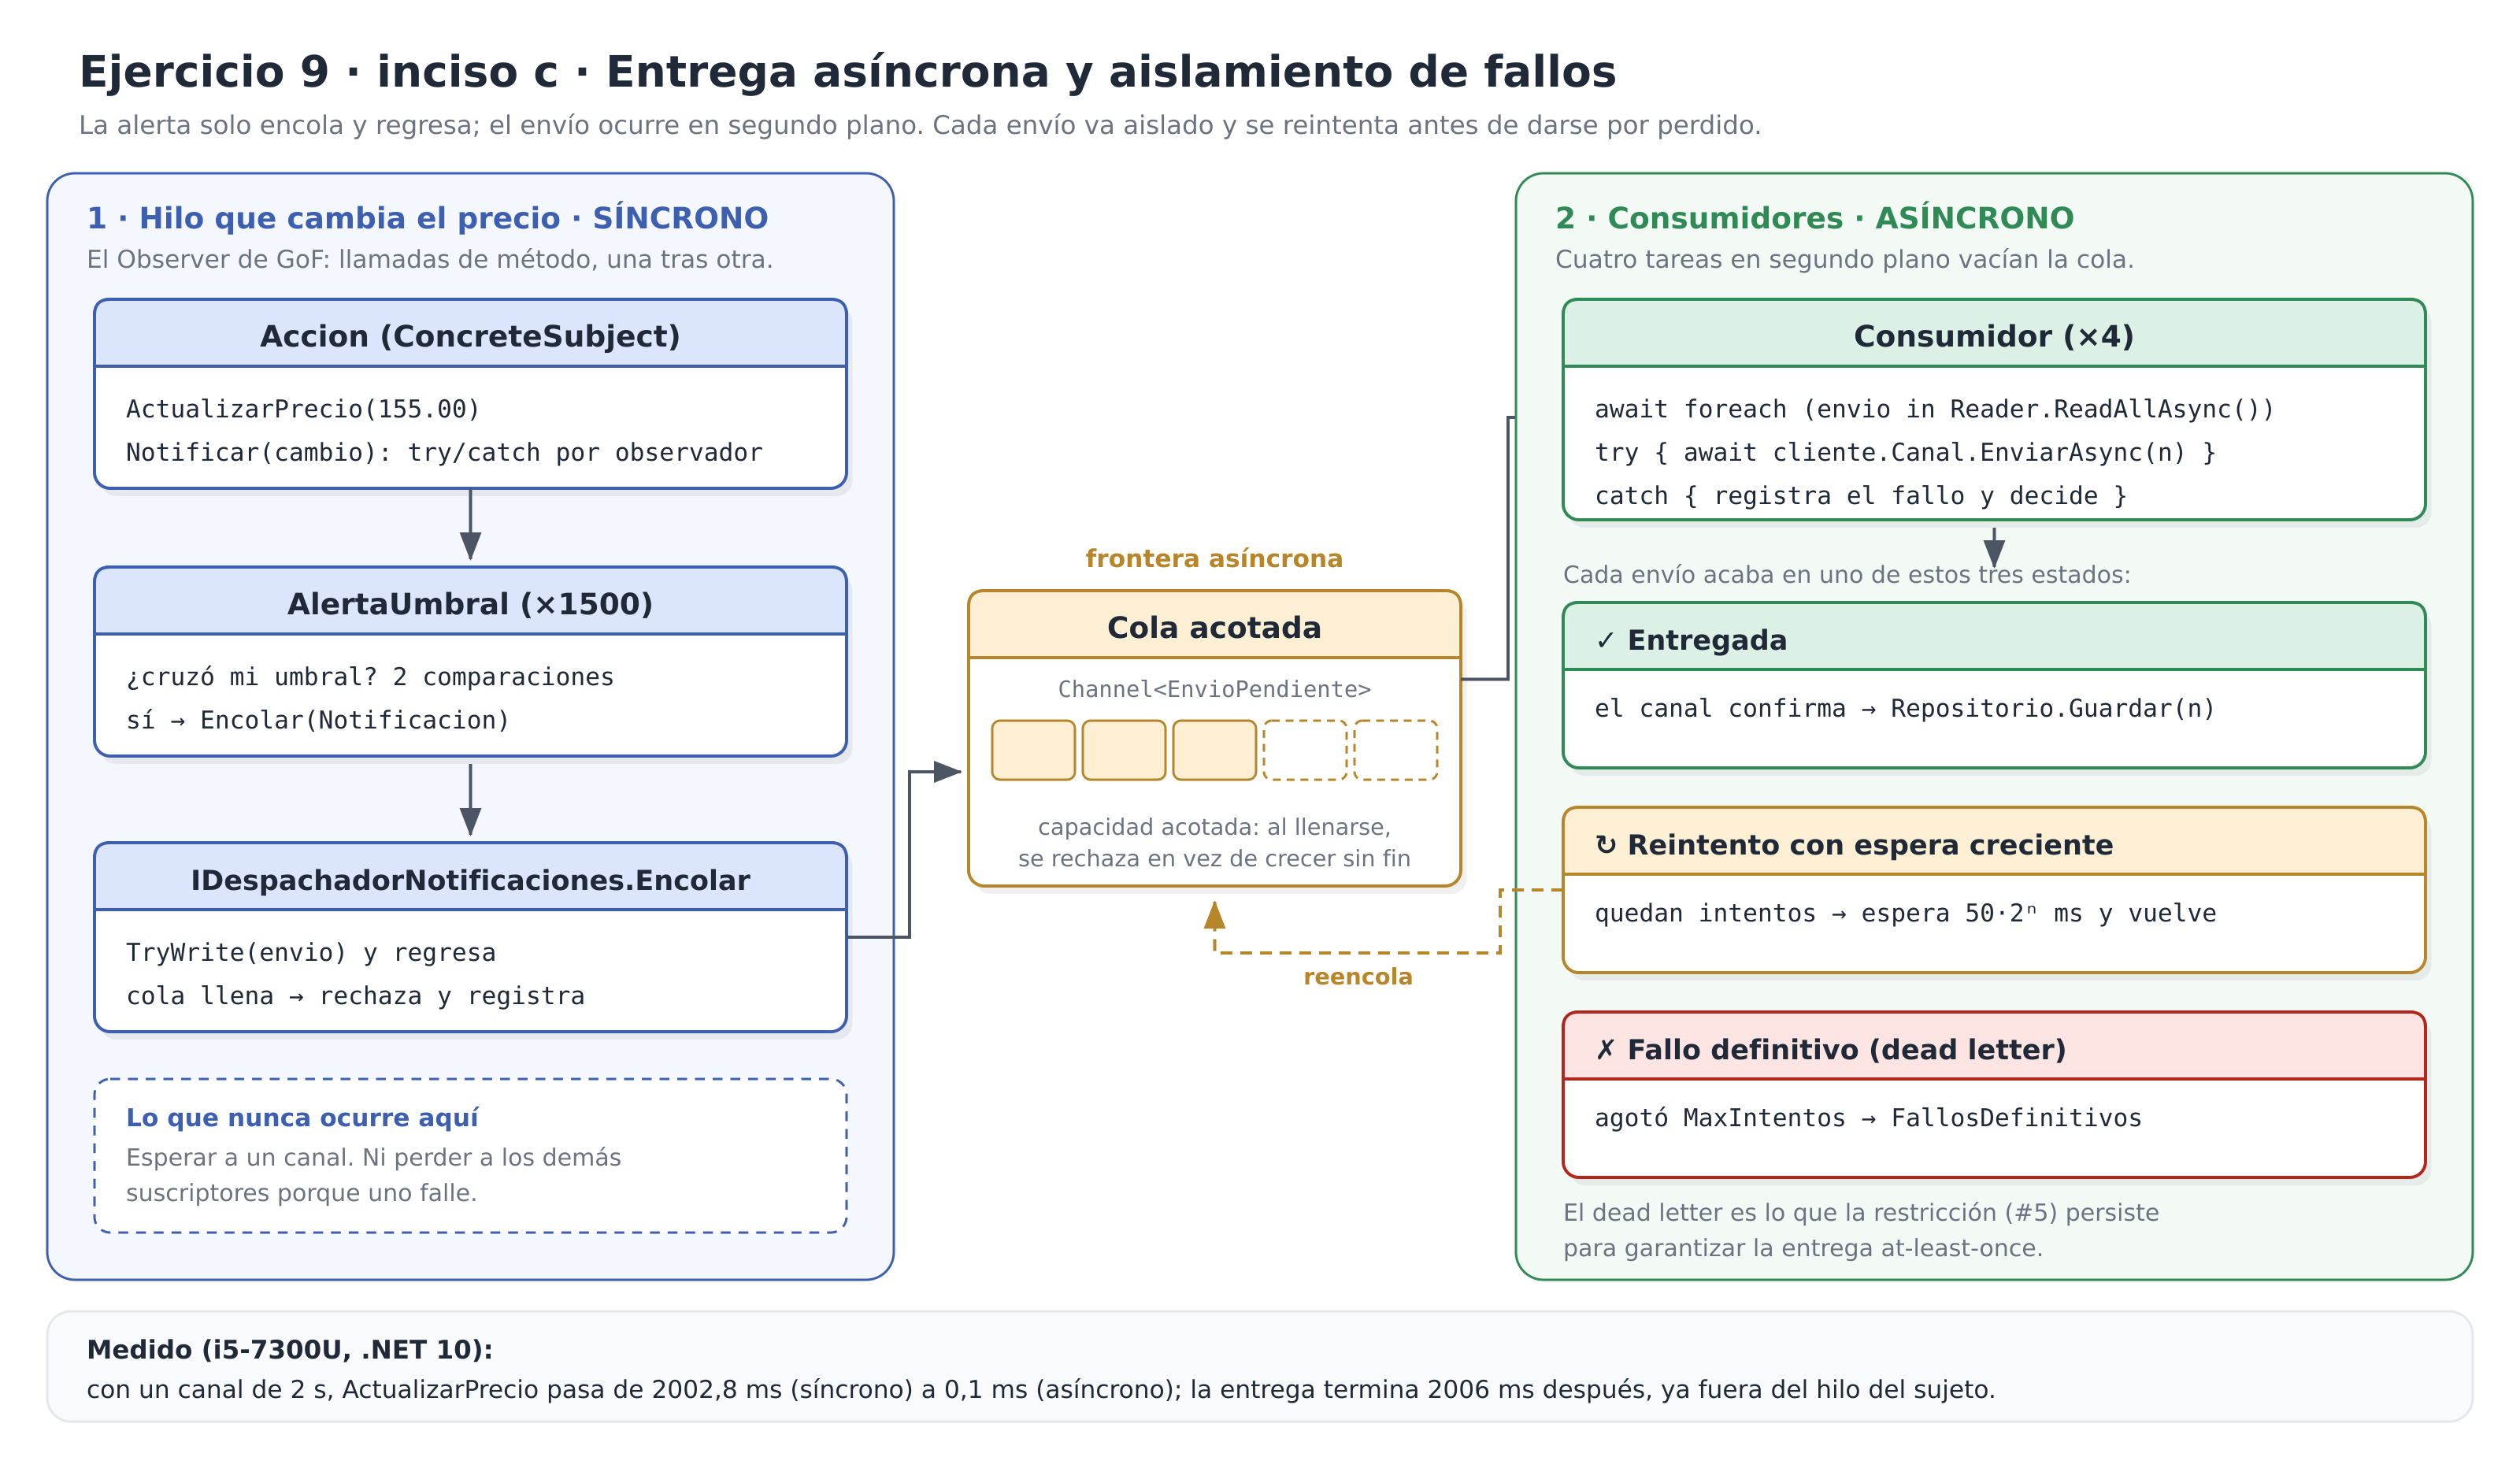
\includegraphics[width=\textwidth]{ejercicio-09-notificaciones-bolsa/diagramas/inciso-c-entrega-asincrona.png}
  \caption{La alerta solo encola; el envío ocurre en segundo plano, aislado y con reintentos.}
  \label{fig:e9-asincrono}
\end{figure}

La alerta sigue haciendo lo mismo que en el inciso b ---decidir si el precio cruzó su umbral
y encolar---, pero ahora \texttt{Encolar} \textbf{solo escribe en la cola y regresa}:

\begin{lstlisting}[basicstyle=\ttfamily\footnotesize, columns=fullflexible, keepspaces=true, caption={Encolar no espera nunca; los consumidores vacían la cola en segundo plano.}]
public void Encolar(Notificacion notificacion)
{
    Interlocked.Increment(ref _enProceso);
    if (_cola.Writer.TryWrite(new EnvioPendiente(notificacion, Intentos: 0)))
    {
        return;
    }

    // Cola llena: esperar aquí sería volver a bloquear al sujeto.
    Interlocked.Decrement(ref _enProceso);
    Interlocked.Increment(ref _rechazadas);
    _registro.Registrar(nameof(DespachadorAsincrono), $"cola llena ({Capacidad})");
}

private async Task ConsumirAsync()
{
    await foreach (EnvioPendiente envio in _cola.Reader.ReadAllAsync())
    {
        await IntentarEnviarAsync(envio);
    }
}
\end{lstlisting}

\begin{table}[H]
\centering
\small
\begin{tabularx}{\textwidth}{>{\raggedright\arraybackslash}p{4.6cm} >{\raggedright\arraybackslash}X}
\toprule
\textbf{Decisión} & \textbf{Por qué} \\
\midrule
\texttt{System.Threading.Channels} y no una \texttt{Queue} con \texttt{lock} &
\texttt{Channel<T>} es una cola productor-consumidor pensada para esto: los consumidores
esperan con \texttt{await} sin consumir CPU, y \texttt{ReadAllAsync} reparte los elementos
entre varios lectores sin sincronizar a mano. \\
\addlinespace
Cola acotada (\texttt{CreateBounded}) y no ilimitada &
Una cola ilimitada convierte una caída del proveedor en memoria creciente hasta agotar el
proceso. Acotada, el sistema tiene que decidir qué hacer cuando se llena; esa decisión es el
\emph{backpressure} del inciso d. \\
\addlinespace
\texttt{TryWrite} y no \texttt{WriteAsync} &
\texttt{WriteAsync} esperaría cuando la cola está llena, y esa espera la pagaría otra vez el
hilo del cambio de precio. Con \texttt{TryWrite} el sujeto nunca espera: en el peor caso la
notificación se rechaza y queda registrada. \\
\bottomrule
\end{tabularx}
\caption{Las tres decisiones de diseño de la cola.}
\end{table}

\paragraph{La medición.}
Medida con \texttt{Stopwatch}, con canales silenciosos (escribir en la consola cuesta más
que el envío simulado y falsearía el resultado):

\begin{table}[H]
\centering
\small
\begin{tabular}{lrrr}
\toprule
\textbf{Escena} & \textbf{Síncrona} & \textbf{Asíncrona} & \textbf{En segundo plano} \\
\midrule
1 canal lento de 2\,s $+$ 2 rápidos & 2002,8\,ms & \textbf{0,1\,ms} & 2006,3\,ms \\
4 canales lentos de 500\,ms, 4 consumidores & 2000,8\,ms & \textbf{0,1\,ms} & 502,0\,ms \\
\bottomrule
\end{tabular}
\caption{Lo que tarda el cambio de precio. Máquina: Intel Core i5-7300U a 2,60\,GHz
(2 núcleos, 4 hilos), 15\,GiB de RAM, Linux, .NET 10.0.113.}
\end{table}

\begin{enumerate}
  \item \textbf{El cambio de precio regresa enseguida} aunque el canal tarde 2\,s: 0,1\,ms
        frente a 2002,8\,ms, cuatro órdenes de magnitud. El trabajo no desapareció, se movió
        de hilo.
  \item \textbf{Varios consumidores solapan los envíos:} cuatro canales de 500\,ms tardan
        502\,ms en total en vez de 2000\,ms. Esto es paralelismo, no un cambio de
        complejidad; de eso se ocupa el inciso d.
\end{enumerate}

\paragraph{Lo que cuesta desacoplar el envío.}
No es gratis, y conviene decirlo:

\begin{itemize}
  \item \textbf{El orden de llegada deja de estar garantizado} (se demuestra más abajo).
  \item \textbf{Aparece concurrencia.} Varios consumidores escriben a la vez en el
        repositorio y en los contadores: de ahí el \texttt{lock} de
        \texttt{RepositorioMemoria} y los \texttt{Interlocked} del despachador.
  \item \textbf{El aviso puede llegar tarde o duplicado.} Si el proceso se reinicia entre el
        envío y la confirmación, la notificación se reenvía: eso es \emph{at-least-once}, y
        es el tema de la restricción.
  \item \textbf{La saturación se hace visible.} Con cola acotada hay que decidir qué pasa
        cuando los cambios de precio llegan más rápido de lo que se puede notificar.
\end{itemize}

\subsubsection{¿Observer es síncrono o asíncrono?}

\paragraph{El Observer de GoF es síncrono.}
Síncrono, y por una razón estructural, no por una elección de implementación. En el código
del patrón, \texttt{Notify} recorre los observadores y llama a \texttt{Update} como una
\textbf{llamada de método ordinaria}: no vuelve de esa llamada hasta que el observador
terminó, y todo ocurre en el hilo de quien cambió el estado del sujeto
(Gamma et al., 1994, p.~335). No hay en el patrón ni cola, ni hilo, ni promesa.

De hecho, el patrón \emph{depende} de eso en un punto: GoF insiste en que el sujeto debe
estar en un estado coherente \textbf{antes} de llamar a \texttt{Notify}
(Gamma et al., 1994, p.~331). Esa recomendación tiene sentido precisamente porque el
observador va a leer el sujeto en ese mismo instante.

\begin{table}[H]
\centering
\small
\begin{tabularx}{\textwidth}{>{\raggedright\arraybackslash}p{5.2cm} >{\raggedright\arraybackslash}X}
\toprule
\textbf{Mecanismo} & \textbf{¿Síncrono?} \\
\midrule
\texttt{Notificar} / \texttt{Actualizar} escritos a mano (nuestro caso) &
Sí: llamada de método en el hilo del sujeto. \\
\addlinespace
\texttt{event} $+$ \texttt{PrecioCambiado?.Invoke(...)} &
Sí: invoca a los suscriptores uno tras otro y en el mismo hilo; si uno lanza, los siguientes
no se ejecutan (el mismo problema de la primera pregunta). \\
\addlinespace
\texttt{IObservable<T>} / \texttt{IObserver<T>} (Rx.NET) &
\texttt{OnNext} también se llama en el hilo del productor, salvo que se interponga
explícitamente un planificador (\texttt{ObserveOn}, \texttt{SubscribeOn}). \\
\bottomrule
\end{tabularx}
\caption{En C\# los mecanismos del lenguaje también son síncronos.}
\end{table}

\paragraph{Puede hacerse asíncrono, pero lo asíncrono no es el patrón.}
La distinción importa para no decir algo falso: lo que se vuelve asíncrono es el
\emph{envío}, no la notificación.

\begin{table}[H]
\centering
\small
\begin{tabularx}{\textwidth}{>{\raggedright\arraybackslash}p{6.5cm} >{\raggedright\arraybackslash}X}
\toprule
\textbf{Paso} & \textbf{¿Síncrono o asíncrono?} \\
\midrule
\texttt{Accion.ActualizarPrecio} $\rightarrow$ \texttt{Notificar} & Síncrono. \\
\texttt{AlertaUmbral.Actualizar} (evalúa el cruce) & Síncrono, en el hilo del sujeto. Es una comparación de dos \texttt{decimal}: barata. \\
\texttt{IDespachadorNotificaciones.Encolar} & Síncrono \textbf{pero no bloqueante}: escribe en la cola y regresa. \\
\texttt{ICanalNotificacion.EnviarAsync} & \textbf{Asíncrono}, en los consumidores de la cola. \\
\bottomrule
\end{tabularx}
\caption{Dónde está exactamente la frontera asíncrona.}
\end{table}

Es decir: el Observer sigue siendo el Observer síncrono de GoF, y la frontera asíncrona se
pone \textbf{dentro del observador}, en lo que este hace con el aviso. Esa es la razón de
que \texttt{AlertaUmbral} no haya cambiado nada de su lógica entre el inciso b y este:
depende de \texttt{IDespachadorNotificaciones}, y cambiar la implementación síncrona por la
asíncrona no la afecta.

\paragraph{Las consecuencias de hacerlo asíncrono.}
El orden de llegada ya no está garantizado. Con tres clientes suscritos en el orden 1, 2, 3
y canales de 300, 100 y 200\,ms:

\begin{lstlisting}[language={}, numbers=none, basicstyle=\ttfamily\scriptsize, columns=fullflexible, keepspaces=true]
--- 3c. El orden de llegada ya no está garantizado ---
  Síncrono (orden de suscripción):
[PUSH → cliente1 (300 ms)] ...
[PUSH → cliente2 (100 ms)] ...
[PUSH → cliente3 (200 ms)] ...
  Asíncrono (orden de respuesta de cada canal):
[PUSH → cliente2 (100 ms)] ...
[PUSH → cliente3 (200 ms)] ...
[PUSH → cliente1 (300 ms)] ...
\end{lstlisting}

\begin{table}[H]
\centering
\small
\begin{tabularx}{\textwidth}{>{\raggedright\arraybackslash}p{2.6cm} >{\raggedright\arraybackslash}p{4.4cm} >{\raggedright\arraybackslash}X}
\toprule
\textbf{Problema} & \textbf{Por qué aparece} & \textbf{Cómo se trata aquí} \\
\midrule
Orden entre avisos & varios consumidores avanzan a distinta velocidad &
No importa en este problema: cada aviso es independiente y lleva su propio precio. Si hiciera
falta orden por cliente, habría que repartir por \texttt{Cliente.Id}. \\
\addlinespace
Estado obsoleto & el precio puede cambiar otra vez antes de que salga el aviso &
Resuelto por el modelo push del inciso a: \texttt{CambioPrecio} y \texttt{Notificacion}
llevan una copia de los precios, así que el consumidor nunca lee un valor más nuevo que el
del evento. \\
\addlinespace
Carreras de datos & varios hilos tocan el repositorio y los contadores &
\texttt{lock} en \texttt{RepositorioMemoria}, \texttt{Interlocked} en los contadores del
despachador. \\
\addlinespace
Duplicados & un reintento puede enviar dos veces si el primer envío llegó pero la
confirmación se perdió &
\texttt{Notificacion} ya tiene \texttt{Id} único (clave de idempotencia). Es la base del
\emph{at-least-once} de la restricción. \\
\addlinespace
Fallos fuera de la pila original & la excepción ya no sube al hilo del sujeto &
Por eso cada envío tiene su \texttt{try/catch} y su registro: en segundo plano, una excepción
no capturada no se ve. \\
\addlinespace
Saturación & los eventos llegan más rápido de lo que se envía &
Cola acotada y rechazo registrado; alternativas en el inciso d. \\
\bottomrule
\end{tabularx}
\caption{Lo que hay que vigilar cuando la entrega deja de ser síncrona.}
\end{table}

\subsubsection{Cambios respecto al código del inciso b}

El diseño del inciso a no cambia: los roles del patrón son los mismos. Lo que se añade está
en la zona de entrega.

\begin{table}[H]
\centering
\small
\begin{tabularx}{\textwidth}{>{\raggedright\arraybackslash}p{6.4cm} >{\raggedright\arraybackslash}X}
\toprule
\textbf{Fichero} & \textbf{Qué es} \\
\midrule
\texttt{Entrega/IDespachadorNotificaciones.cs} & \textbf{Nuevo.} Lo único que la alerta necesita: \texttt{Encolar}. \\
\texttt{Entrega/DespachadorAsincrono.cs} & \textbf{Nuevo.} Cola acotada, consumidores, reintentos y dead letter. \\
\texttt{Entrega/EnvioPendiente.cs} & \textbf{Nuevo.} La notificación más el número de intentos. \\
\texttt{Entrega/CanalLento.cs},\newline\texttt{Entrega/CanalQueFalla.cs} & \textbf{Nuevos.} Decoradores para simular un proveedor lento y uno caído. \\
\texttt{Entrega/CanalSilencioso.cs} & \textbf{Nuevo.} Canal que solo cuenta, para no falsear las mediciones. \\
\texttt{Diagnostico/IRegistroFallos.cs},\newline\texttt{Diagnostico/RegistroFallos.cs} & \textbf{Nuevos.} Donde se anota cada fallo aislado. \\
\texttt{Observer/Accion.cs} & \textbf{Modificado.} \texttt{Notificar} aísla a cada observador. \\
\texttt{Observer/AlertaUmbral.cs} & \textbf{Modificado.} Depende de la interfaz, no de la clase concreta. Su lógica no cambió. \\
\texttt{Entrega/DespachadorNotificaciones.cs} & \textbf{Modificado.} Implementa la nueva interfaz; su comportamiento es el mismo. \\
\texttt{Demos/SimulacionBolsa.cs} & \textbf{Movido} desde \texttt{Program.cs}, sin cambios de lógica. \\
\texttt{Demos/AccionSinAislamiento.cs} & \textbf{Nuevo.} El Subject clásico, solo para la demostración. \\
\texttt{Demos/DemoAsincrona.cs} & \textbf{Nuevo.} La demostración de este inciso. \\
\bottomrule
\end{tabularx}
\caption{Ficheros nuevos y modificados.}
\end{table}

La simulación del inciso b sigue dando exactamente los mismos resultados (417 avisos, 306
clientes, 0 avisos tras la desuscripción).

\subsubsection{Pruebas unitarias}

\texttt{dotnet test} ejecuta \textbf{20 pruebas, todas correctas}; 9 son de este inciso:

\begin{table}[H]
\centering
\small
\begin{tabularx}{\textwidth}{>{\raggedright\arraybackslash}p{6.1cm} >{\raggedright\arraybackslash}X}
\toprule
\textbf{Prueba} & \textbf{Qué comprueba} \\
\midrule
\texttt{ElBucleClasicoSeCorta\_Cuando\-UnObservadorFalla} & Sobre el Subject clásico: el primero recibe, el último no, y la excepción sale de \texttt{ActualizarPrecio} \\
\texttt{UnClienteNoNotificableNoImpide\-QueLosDemasReciban} & Misma escena con \texttt{Accion}: los dos clientes sanos reciben y el fallo queda registrado \\
\texttt{ElPrecioSeActualizaAunque\-UnObservadorFalle} & Un fallo de entrega no corrompe la cotización \\
\texttt{ReintentaYEntrega\_Cuando\-ElCanalSeRecupera} & Canal que falla 2 veces: 2 reintentos, 3 intentos, entregada \\
\texttt{DaPorPerdidaLaNotificacion\_\-TrasAgotarLosIntentos} & Canal siempre caído: 3 intentos y dead letter; no se guarda como entregada \\
\texttt{UnCanalCaidoNoImpideLa\-EntregaDeLosDemasClientes} & Aislamiento por envío, no solo por observador \\
\texttt{EntregaEnSegundoPlanoTodasLas\-NotificacionesEncoladas} & 50 notificaciones encoladas se entregan todas \\
\texttt{ElCambioDePrecioNoEspera\-AlCanalLento} & Con un canal de 1\,s, \texttt{ActualizarPrecio} regresa en menos de 500\,ms y nada se ha entregado todavía; tras vaciar la cola, sí \\
\texttt{RechazaSinBloquear\_Cuando\-LaColaEstaLlena} & 100 avisos con capacidad 1: hay rechazos, encolar no espera, y cada aviso acaba entregado o rechazado \\
\bottomrule
\end{tabularx}
\caption{Las pruebas del inciso c.}
\end{table}
